\section{The algebraic locus in a family}\label{sec:loci}

\begin{definition}\label{def:algloc}
Let $\pi\colon\mathcal{X}\to S$ be a smooth projective morphism to a smooth connected complex quasi-projective variety, and let $\xi$ be a global section of $R^{2p}\pi_{*}\QQ$ that is a Hodge class at one point. The algebraic locus of $\xi$ is the set $\Sigma(\xi)$ of $s\in S$ at which $\xi_{s}\in H^{2p}(\mathcal{X}_{s})$ is algebraic.
\end{definition}

By the theorem of the fixed part \cite{Del71,And92}, the flat sections of a polarisable variation form a sub-Hodge structure, constant along $S$; so $\xi_{s}$ is a Hodge class at every point once it is one somewhere.

\begin{lemma}[Dichotomy]\label{lem:dichotomy}
\leavevmode
\begin{enumerate}[label=\textup{(\roman*)},leftmargin=2.4em,itemsep=2pt]
\item $\Sigma(\xi)$ is a countable union of Zariski closed subsets of $S$.
\item Either $\Sigma(\xi)=S$ or $\Sigma(\xi)$ is meagre in $S^{\mathrm{an}}$.
\item The following are equivalent: $\Sigma(\xi)=S$; $\Sigma(\xi)$ has an interior point; $\Sigma(\xi)$ is not meagre; $\xi_{s}$ is algebraic for the very general $s$. If $\Sigma(\xi)$ is dense they are equivalent to $\Sigma(\xi)$ being closed.
\end{enumerate}
\end{lemma}

\begin{proof}
(i) Fix a relatively ample line bundle on $\mathcal{X}$. For a Hilbert polynomial $P$ the relative Hilbert scheme $\mathrm{Hilb}^{P}(\mathcal{X}/S)$ is projective over $S$ \cite{Gro61}, and the class of the fibre of the universal family in $H^{2p}(\mathcal{X}_{s})$ is locally constant on each connected component of it, since a flat family of subschemes over a connected base has locally constant cycle class. A rational combination $\sum_{i}a_{i}[Z_{i}]$ equal to $\xi_{s}$ is a point of a fibre product $\prod_{S}\mathrm{Hilb}^{P_{i}}(\mathcal{X}/S)$, projective over $S$ and with countably many connected components; on each component the condition $\sum a_{i}[Z_{i}]=\xi$ is either empty or holds throughout, because both sides are flat sections. So $\Sigma(\xi)$ is the union, over the countably many tuples $(P_{i},a_{i})$ and components, of images of proper morphisms to $S$, each Zariski closed.

(ii) A countable union of proper Zariski closed subsets of an irreducible $S$ has empty interior in $S^{\mathrm{an}}$, and each is closed, so the union is meagre; if one of the closed sets is $S$ itself, $\Sigma(\xi)=S$.

(iii) By the Baire category theorem $S^{\mathrm{an}}$ is not meagre in itself, so $\Sigma(\xi)=S$ excludes meagreness, and a set with an interior point is not meagre; by (ii) not meagre forces $\Sigma(\xi)=S$. The complement of a countable union of proper closed subvarieties is the very general locus, so algebraicity at the very general point means that one of the closed sets is all of $S$. A dense set that is also closed is $S$.
\end{proof}

\begin{lemma}[Points of CM type are dense]\label{lem:cmdense}
Let $G$ be a connected reductive group over $\QQ$, $u_{0}\colon U(1)\to G_{\RR}$ a homomorphism and $\cD$ the orbit of $u_{0}$ under conjugation by $G(\RR)^{+}$. The points $u\in\cD$ for which $u(U(1))$ lies in the real points of a maximal torus of $G$ defined over $\QQ$ are dense in $\cD$.
\end{lemma}

\begin{proof}
Let $u_{1}\in\cD$ and $W$ a neighbourhood of $u_{1}$. A maximal torus $T_{1}$ of $G_{\RR}$ contains $u_{1}(U(1))$, since the centraliser of that compact torus is reductive and connected. Pick a regular element $Y_{1}$ in the Lie algebra $\mathfrak{t}_{1}$ of $T_{1}$. The map $(g,Y)\mapsto\mathrm{Ad}(g)Y$ from $G(\RR)^{+}\times\mathfrak{t}_{1}$ to $\mathfrak{g}_{\RR}$ is submersive at $(1,Y_{1})$ because $\mathfrak{g}_{\RR}=\mathfrak{t}_{1}\oplus[\mathfrak{g}_{\RR},Y_{1}]$, so the image of a small neighbourhood $N_{1}\times N_{2}$, with $N_{1}u_{1}N_{1}^{-1}\subseteq W$ and $N_{2}$ made of regular elements, contains an open set of $\mathfrak{g}_{\RR}$, hence a rational point $Y=\mathrm{Ad}(g)Y'$. The identity component $T$ of the centraliser of the rational regular semisimple $Y$ is a maximal torus over $\QQ$ with $T_{\RR}=gT_{1}g^{-1}$, and $u=gu_{1}g^{-1}\in W$ has $u(U(1))\subseteq T_{\RR}$.
\end{proof}

When $G=\Hg(A)$ and $u$ is the Hodge cocharacter of an abelian variety $A$, the condition of the lemma says that $\Hg(A)$ lies in a $\QQ$-torus, and then $A$ is of CM type: a maximal $\QQ$-torus of $\mathrm{GL}(H^{1}(A))$ containing it is the unit group of a commutative semisimple algebra $L$ of dimension $2\dim A$ commuting with $\Hg(A)$, and the commutant of $\Hg(A)$ is $\End^{0}(A)$.

\begin{proposition}[A family with a CM member through every Hodge class]\label{prop:cmfamily}
Let $A_{0}$ be an abelian variety and $\gamma$ a Hodge class on it. There are a polarised abelian scheme $\pi\colon\cA\to S$ over a smooth connected quasi-projective base, a flat section $\xi$ of $R^{2p}\pi_{*}\QQ$, a point $s_{0}$ with $\cA_{s_{0}}\cong A_{0}$ and $\xi_{s_{0}}=\gamma$, and a point $c$ with $\cA_{c}$ of CM type; the points of CM type are dense in $S$.
\end{proposition}

\begin{proof}
Let $G=\Hg(A_{0})$, let $u_{0}$ be the Hodge cocharacter of $A_{0}$ and $\cD$ its $G(\RR)^{+}$-orbit. Every $u\in\cD$ defines a polarisable Hodge structure of weight one on $H^{1}(A_{0})$ with Hodge group contained in $G$, so an abelian variety $A_{u}$ up to isogeny; fixing the lattice $H^{1}(A_{0},\ZZ)$, the polarisation of $A_{0}$ and a level structure of level $N\ge3$, the quotient $S=\Gamma\backslash\cD$ by a neat congruence subgroup $\Gamma\subseteq G(\QQ)$ is a smooth quasi-projective variety carrying a polarised abelian scheme with these fibres \cite{Mum69,Del71}. The class $\gamma$ is invariant under $G$, so it is a flat section $\xi$ of $R^{2p}\pi_{*}\QQ$, and $\xi_{s_{0}}=\gamma$ at the image $s_{0}$ of $u_{0}$. By Lemma~\ref{lem:cmdense} the points of CM type are dense in $\cD$, hence in $S$.
\end{proof}

\begin{theorem}[\Fii{} is propagation from CM points]\label{thm:propagation}
The following are equivalent.
\begin{enumerate}[label=\textup{(\roman*)},leftmargin=2.4em,itemsep=2pt]
\item \Fii{}.
\item $\AB$.
\item For every polarised abelian scheme $\pi\colon\cA\to S$ and every flat Hodge class $\xi$, algebraicity of $\xi_{s}$ at one point $s$ forces $\Sigma(\xi)=S$.
\item The same for the points $s$ of CM type.
\item For every $\pi$, $\xi$ with $\xi_{c}$ algebraic at a point $c$ of CM type, $\Sigma(\xi)$ has an interior point.
\end{enumerate}
\end{theorem}

\begin{proof}
(i) and (ii) are Theorem~\ref{thm:f2isab}. If (ii) holds, $\xi_{t}$ is a Hodge class at every $t$ by the theorem of the fixed part and algebraic by (ii), so (iii) holds; (iv) is a case of (iii), and (iv) and (v) are equivalent by Lemma~\ref{lem:dichotomy}(iii).

Assume (iv). Let $F$ be a CM field and $n\ge2$. The family of abelian varieties of split Weil type for $F$ over its Shimura variety is a polarised abelian scheme on which the Weil classes are flat sections, and by \cite[Thm.~1.1(i)]{BMB26} they are algebraic at a member isogenous to a product of abelian varieties with complex multiplication by $F$, a member of CM type; so by (iv) they are algebraic on every member, and by pull-back along an $F$-linear isogeny on every abelian variety of split Weil type for $F$. By Andr\'e's theorem, in the form Milne gives it \cite[Thm.~1 and \S5]{Mil20}, every Hodge class on an abelian variety of CM type is a sum of pull-backs, along homomorphisms, of Weil classes of abelian varieties of split Weil type; so $\AB$ holds for every abelian variety of CM type. Now let $A_{0}$ be any abelian variety and $\gamma$ a Hodge class on it, and take $\pi$, $\xi$, $s_{0}$, $c$ from Proposition~\ref{prop:cmfamily}. Then $\xi_{c}$ is algebraic, (iv) gives $\Sigma(\xi)=S$, and $\gamma=\xi_{s_{0}}$ is algebraic. This is (ii).
\end{proof}

\begin{proposition}[The Weil classes]\label{prop:weil-dense}
For every CM field $F$, every $n\ge2$ and every discriminant, the algebraic locus of the Weil classes in the polarised period domain $\cD_{F}$ contains an explicit point of CM type and is dense, and it is either $\cD_{F}$ or meagre.
\end{proposition}

\begin{proof}
This is \cite[Thm.~1.1]{BMB26}, items (i) to (iii). The density is the Hecke orbit of the base point: the group $G_{F}(\QQ)$ of the unitary group of the hermitian form acts on $\cD_{F}$ through $F$-linear isogenies that preserve the polarisation up to a scalar, hence preserve the algebraicity of the Weil classes, and its closure contains $G_{F}(\RR)^{+}$, which acts transitively. The dichotomy is Lemma~\ref{lem:dichotomy}.
\end{proof}

\begin{proposition}[\Fiii{} and the abelian part]\label{prop:abpart}
Let $H^{2p}_{\mathrm{ab}}(X)\subseteq H^{2p}(X)$ be the sum of the images of all maps $\Gamma_{*}\colon H^{k}(B)\to H^{2p}(X)$ with $B$ abelian and $\Gamma$ an algebraic cycle on $B\times X$. Then $H^{2p}_{\mathrm{ab}}(X)$ is a sub-Hodge structure, $\Ab^{p}(X)=\Hdg^{p}(X)\cap H^{2p}_{\mathrm{ab}}(X)$, and \Fiii{} holds for $X$ in degree $2p$ if and only if a Hodge complement $T^{2p}_{\mathrm{ab}}(X)$ of $H^{2p}_{\mathrm{ab}}(X)$ carries no nonzero Hodge class.
\end{proposition}

\begin{proof}
Each $\Gamma_{*}$ is a morphism of Hodge structures, so its image and the sum of finitely many images, which is all of $H^{2p}_{\mathrm{ab}}(X)$ by dimension, are sub-Hodge structures. A Hodge class in $H^{2p}_{\mathrm{ab}}(X)$ is $\sum\Gamma_{j*}y_{j}$, and the argument of Proposition~\ref{prop:f3prime-known}(i) replaces each $y_{j}$ by a Hodge class; so $\Ab^{p}(X)=\Hdg^{p}(X)\cap H^{2p}_{\mathrm{ab}}(X)$. A Hodge complement exists because the Hodge group is reductive, and the Hodge classes of $H^{2p}(X)$ are the direct sum of those of the two summands, which gives the last assertion.
\end{proof}

Theorem~\ref{thm:intro-loci} is Lemma~\ref{lem:dichotomy}, Theorem~\ref{thm:propagation}, Proposition~\ref{prop:weil-dense} and Proposition~\ref{prop:abpart}. Figure~\ref{fig:locus} draws the locus of Proposition~\ref{prop:weil-dense}.

\begin{figure}[t]
\centering
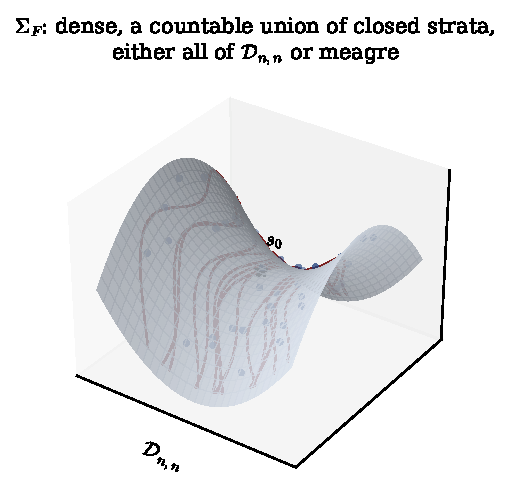
\includegraphics[width=0.95\columnwidth]{figures/fig_locus}
\caption{The period domain $\cD_{n,n}$ of a Weil family as a surface. The star is the CM base point, the dots and curves are strata of the algebraic locus, dense by the Hecke orbit. The locus is a countable union of closed strata; it is either the whole surface or meagre.}
\label{fig:locus}
\end{figure}

Both statements are now of one shape. There is a dense set of points at which the class is algebraic by an explicit cycle; the locus is a countable union of closed strata; the statement is that this union is not meagre, that is, that algebraicity propagates from the dense set. The rest of the paper goes to the first point where the propagation is not known and builds the object that would carry it.
